% Section content template for individual Educative lessons
% This file contains the actual content for a specific section
% Generated from Educative API section content

% Section: Activity Diagram for the Library Management System
% Section ID: 6368808088633344
% Section Slug: activity-diagram-for-the-library-management-system
% Generated: 2025-12-11T15:13:35.280995

Activity diagrams are a great way to visualize the flow of messages from one activity to another in the system. There can be different activity diagrams that we can create for our LMS(Library Management System). In this lesson, we will create activity diagrams for the following three activities:

\begin{itemize}
\item
\protect\phantomsection\label{XjMxpaa4nrzIzEyBfb7xG}
Check out a book from the library.
\item
\protect\phantomsection\label{6ha9UjvexcOEWha8jIh83}
Return a book to the library.
\item
\protect\phantomsection\label{kVHkayzgJEjJeg6f-S5pQ}
\textbf{Activity challenge:} Renew a book from the library.
\end{itemize}

\subsection{Check out a book from the library}\label{c1z3pjkp2cfwqY1SwP0IL}
\\
The following are the states and actions involved in this activity diagram.

\subsubsection{States}\label{pH_MAFYDUiS35LNDrME4A}
\\
\textbf{Initial state:} The member selects a book and initiates checkout.
\\
\textbf{Final state:} There are two final states present in this activity diagram, shown below:

\begin{itemize}
\item
\protect\phantomsection\label{LENao63ZprXOMOwF0g-Ee}
The member completes the checkout process successfully, and the book will be allocated to the member.
\item
\protect\phantomsection\label{IPIkGEPjxjFPTV2GPF74r}
An error occurred during checkout due to book unavailability, or the book limit was exceeded.
\end{itemize}

\subsubsection{Actions}\label{nv8Cna8fcsGiR89wFzkrf}
\\
The member selects a book and enters the ID. The system performs a few checks, such as book availability, the member's maximum limit, and book reservations. If all checks are clear, the book will be issued. Otherwise, the system will show an error message.
\\
The activity diagram of a library book checkout is given below based on the order shown above.

\begin{figure}[htbp]
 \centering
 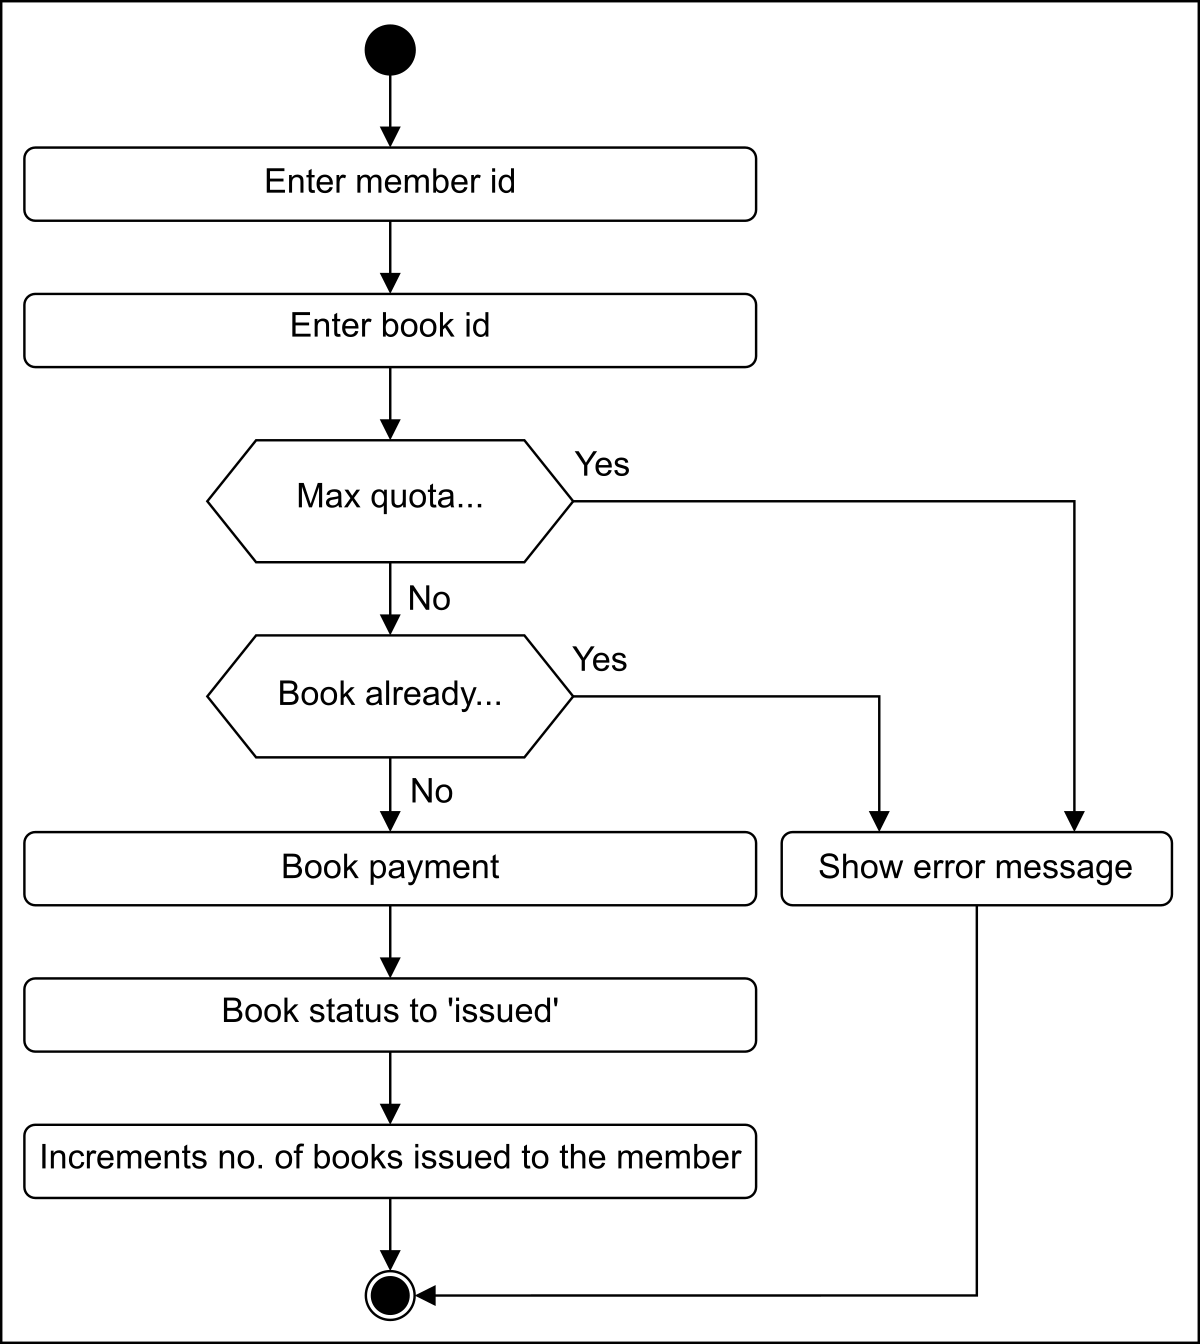
\includegraphics[width=0.5\textwidth]{Images/chapter_9/section_6368808088633344/6746344057470976.png}
 \caption{The activity diagram to check out a book from the library}
\end{figure}

\subsection{Return a book to the library}\label{rVcAqNnNEhcO5EdRgNP2b-2}
\\
The following are the states and actions involved in this activity diagram.

\subsubsection{States}\label{erckDk952KPFVLQOJ-B9y}
\\
\textbf{Initial state:} The member returns a book to the library.
\\
\textbf{Final state:} There are two final states present in this activity diagram, shown below:

\begin{itemize}
\item
\protect\phantomsection\label{ZwbOpRO0i9hqn9y7R4IIu}
The member completes the return process and pays a fine, if any.
\item
\protect\phantomsection\label{0gxkjfHAAWiWpzLDBBXDw}
The system allocates a book to someone who reserved that book.
\end{itemize}

\subsubsection{Actions}\label{77mZsyrU-7k79t9ouYhVX}
\\
The member enters the book ID. The system checks if the book is returned within the due date, and the member pays a fine, if any. Then , the book is allocated to someone who has reserved it.
\\
Based on the order above, the activity diagram below demonstrates returning a book to the library.

\begin{figure}[htbp]
 \centering
 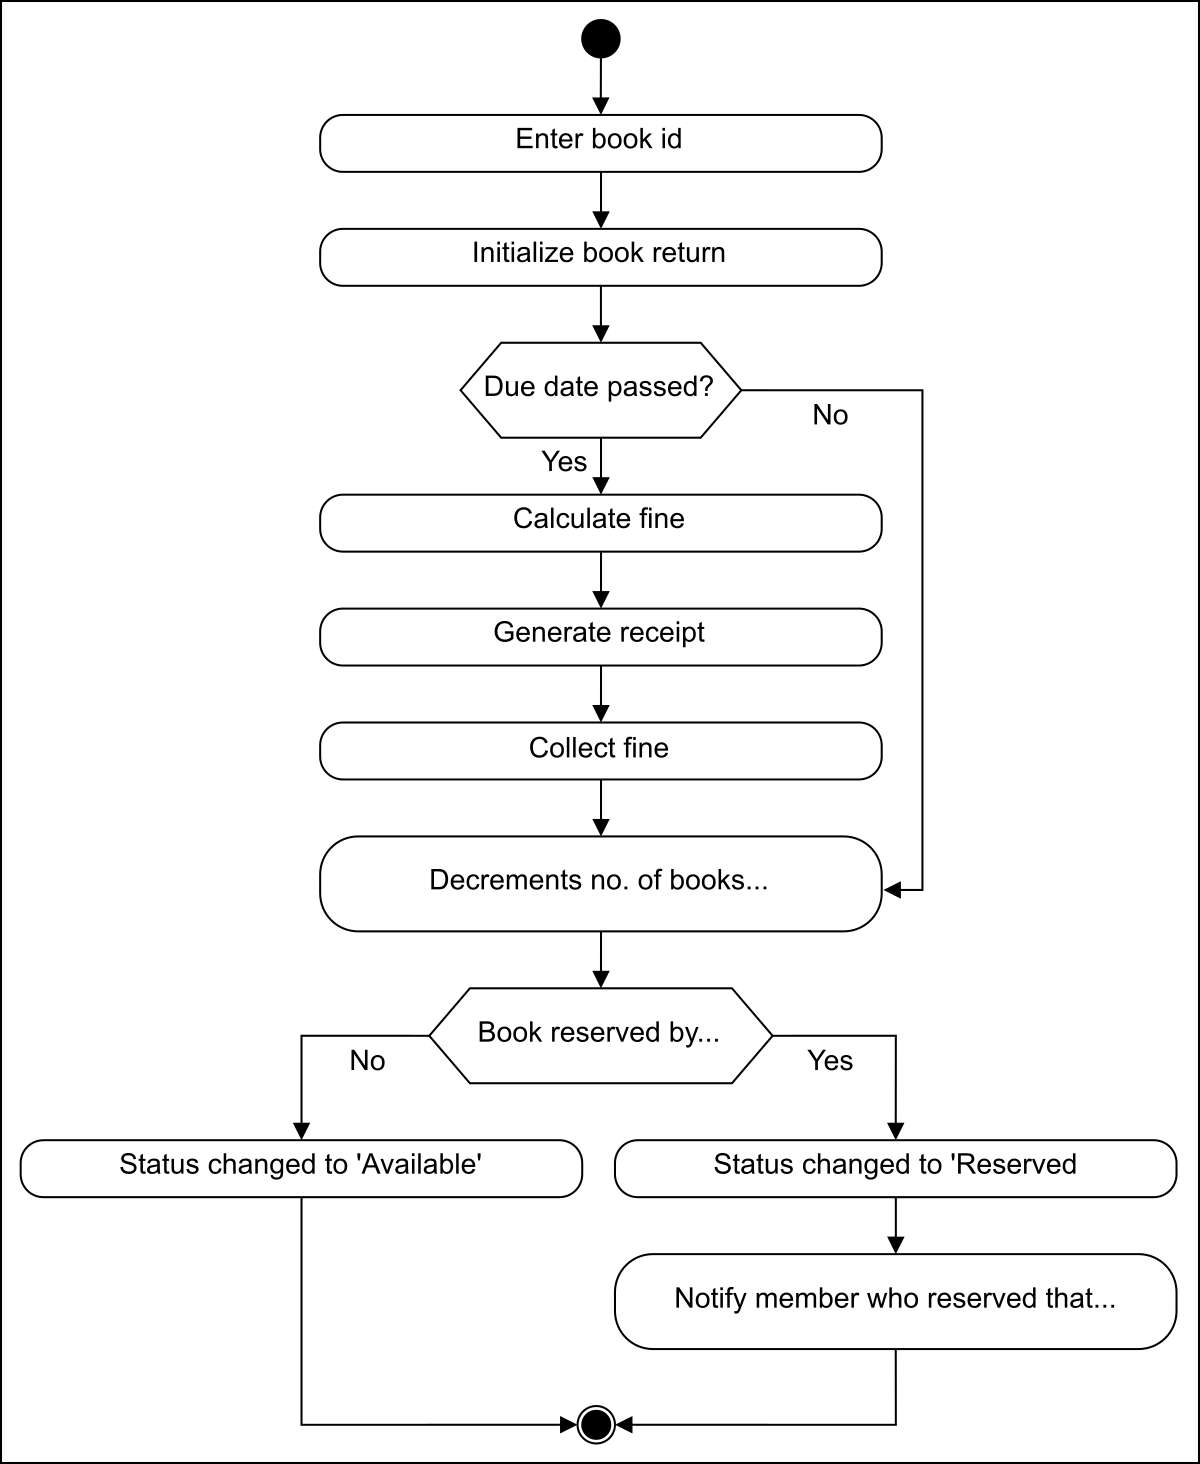
\includegraphics[width=0.5\textwidth]{Images/chapter_9/section_6368808088633344/5020274610405376.png}
 \caption{The activity diagram for returning a book to the library}
\end{figure}

\subsection{Activity challenge: Renew a book from the library}\label{qQ8UiLDWEEf6Cnibbq9TJ}
\\
You will create an activity diagram of a member renewing a book from the library.
\\
The skeleton of the activity diagram given below demonstrates a customer looking for book renewal from the library.

\begin{figure}[htbp]
 \centering
 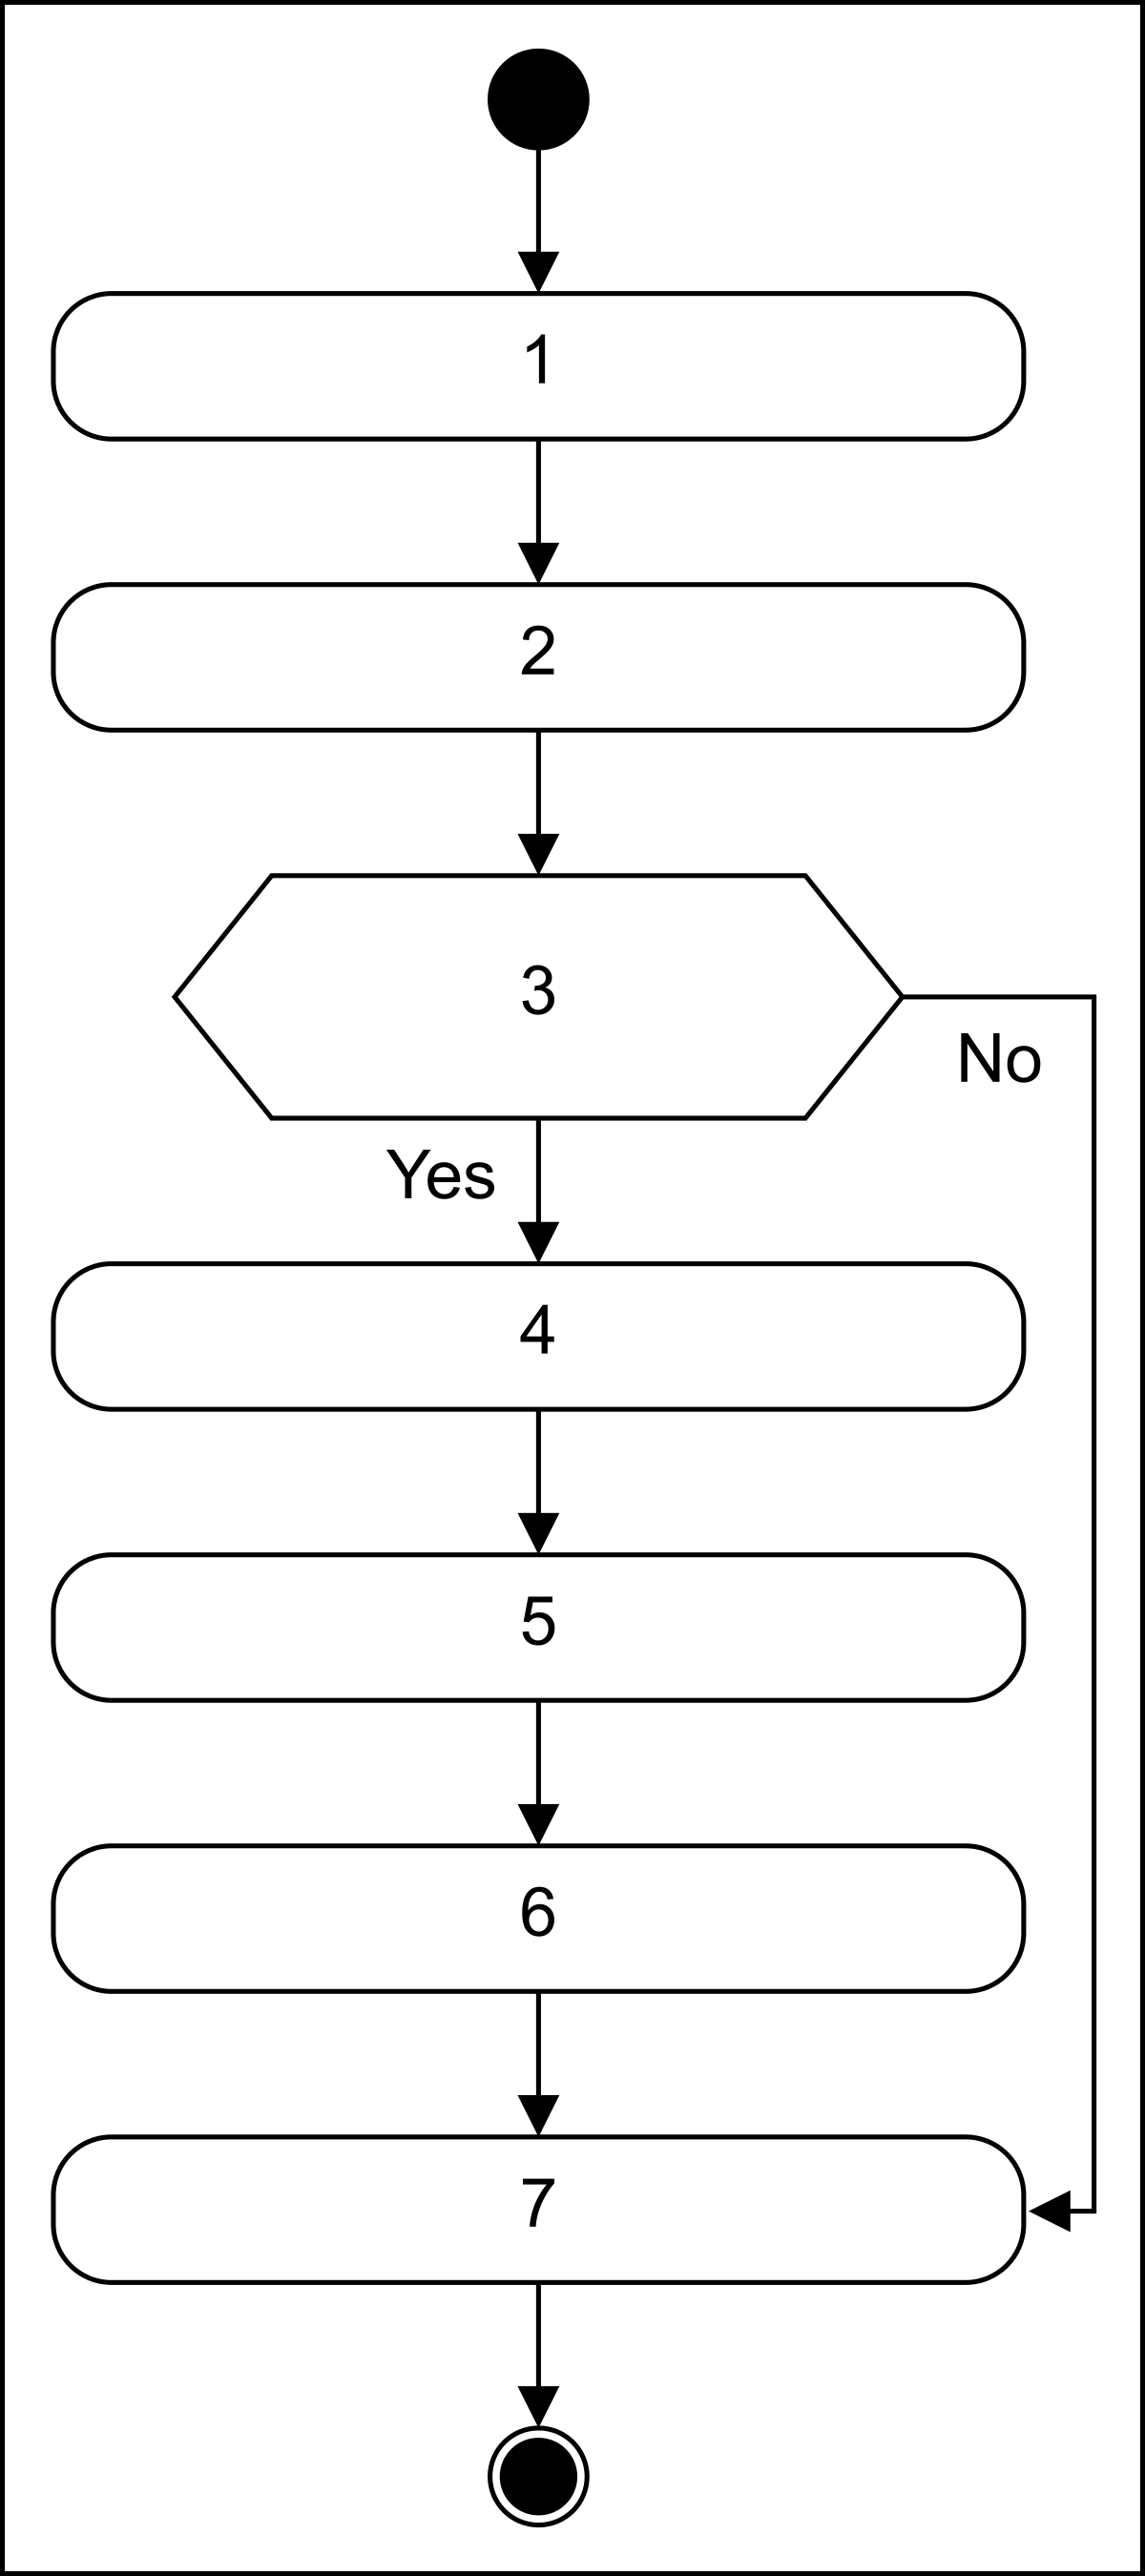
\includegraphics[width=0.5\textwidth]{Images/chapter_9/section_6368808088633344/6071839928614912.png}
 \caption{The activity diagram for renewing a book at the library}
\end{figure}

Notice that the actions in the above diagram are numbered from 1 to 7. The slots below represent the activities, and the arrows represent the flow from one activity to another. Can you rearrange the slots provided below in the correct order they should appear in the activity diagram above?
\\
Based on the description above, can you fill in the missing slots in the activity diagram with the correct sequence of actions?
\begin{quote}
\textbf{Note:} If you're stuck, click the ``Show Solution'' button.
\end{quote}

Alternatively, you can click the ``Show complete diagram'' button below to see the complete activity diagram.

We've looked at some of our library management system's activity diagrams. The next lesson will present the code for our designed classes in some of the most popular languages.

% End of section content